                  %% ----------------------------------------------------------------
%% Thesis.tex -- MAIN FILE (the one that you compile with LaTeX)
%% ---------------------------------------------------------------- 


% Set up the document
\documentclass[a4paper, 11pt, oneside]{Thesis}  % Use the "Thesis" style, based on the ECS Thesis style by Steve Gunn
\graphicspath{Figures/}  % Location of the graphics files (set up for graphics to be in PDF format)
\usepackage{subcaption}  % add this in preamble
% Include any extra LaTeX packages required
\usepackage[square, numbers, comma, sort&compress]{natbib}  % Use the "Natbib" style for the references in the Bibliography
\usepackage{verbatim}  % Needed for the "comment" environment to make LaTeX comments
\usepackage{vector}  % Allows "\bvec{}" and "\buvec{}" for "blackboard" style bold vectors in maths
\usepackage{titlesec}
% Pretty tables + stacked values with p-values beneath
\usepackage{booktabs,makecell}
\newcommand{\pv}[1]{\footnotesize(#1)}                   % p-value style
\newcommand{\valp}[2]{\makecell[c]{#1 \\ \pv{#2}}}       % value on top, (p) below
\usepackage{graphicx}
\usepackage{caption}   % for \captionof

\hypersetup{urlcolor=blue, colorlinks=true}  % Colours hyperlinks in blue, but this can be distracting if there are many links.

%% ----------------------------------------------------------------
\begin{document}
\frontmatter      % Begin Roman style (i, ii, iii, iv...) page numbering

% Set up the Title Page
\title  {Sentiment-Managed Factor Portfolios}


%\date       {\today}
%\subject    {}
%\keywords   {}

\maketitle
%% ----------------------------------------------------------------

\setstretch{1.3}  % It is better to have smaller font and larger line spacing than the other way round

% Define the page headers using the FancyHdr package and set up for one-sided printing
\fancyhead{}  % Clears all page headers and footers
\rhead{\thepage}  % Sets the right side header to show the page number
\lhead{}  % Clears the left side page header

\pagestyle{fancy}  % Finally, use the "fancy" page style to implement the FancyHdr headers

%% ----------------------------------------------------------------


% The Abstract Page
%\addtotoc{Abstract}  % Add the "Abstract" page entry to the Contents
%\abstract{
%\addtocontents{toc}{\vspace{1em}}  % Add a gap in the Contents, for aesthetics

%The standard risk–return trade-off implies that higher risk should earn higher return. Moreira and Muir (2017) challenged this by showing that volatility-timing of factor portfolios yields positive alpha. Building on their framework, I test whether such gains survive strict out-of-sample implementation and whether Economic Policy Uncertainty (EPU) can serve as an alternative timing signal. Using U.S. data (1963–2024), I construct volatility- and EPU-managed Fama–French factors and evaluate performance with Sharpe ratios, Ledoit–Wolf tests, and alpha regressions. Results show only modest improvements and no statistically reliable outperformance. Both volatility- and EPU-based scaling behave as risk-control overlays rather than sources of robust alpha.

%}

%\vspace{1em} % a little vertical space
%\clearpage  % Abstract ended, start a new page
%% ----------------------------------------------------------------

\setstretch{1.3}  % Reset the line-spacing to 1.3 for body text (if it has changed)

\pagestyle{fancy}  %The page style headers have been "empty" all this time, now use the "fancy" headers as defined before to bring them back


%% ----------------------------------------------------------------
%\lhead{\emph{Contents}}  % Set the left side page header to "Contents"
%\tableofcontents  % Write out the Table of Contents

%% ----------------------------------------------------------------
%\lhead{\emph{List of Figures}}  % Set the left side page header to "List if Figures"
%\listoffigures  % Write out the List of Figures

%% ----------------------------------------------------------------
%\lhead{\emph{List of Tables}}  % Set the left side page header to "List of Tables"
%\listoftables  % Write out the List of Tables

%% ----------------------------------------------------------------

%% ----------------------------------------------------------------

%% ----------------------------------------------------------------



\mainmatter	  % Begin normal, numeric (1,2,3...) page numbering
\pagestyle{fancy}  % Return the page headers back to the "fancy" style
%\usepackage{natbib}

% Include the chapters of the thesis, as separate files
% Just uncomment the lines as you write the chapters
% Reduce space before chapter titles and keep them compact
% Show only the title, no "Chapter 1"
\titleformat{\chapter}[display]
  {\huge\bfseries}{}{0pt}{\Huge}
\titlespacing*{\chapter}{0pt}{-40pt}{10pt}


\titleformat{\chapter}[hang]{\huge\bfseries}{}{0pt}{\Huge}
\titlespacing*{\chapter}{0pt}{0pt}{10pt}

% Remove automatic new page before chapters
\makeatletter
\renewcommand{\chapter}{\@startsection{chapter}{0}{0pt}%
  {-3.5ex plus -1ex minus -.2ex}%
  {2.3ex plus.2ex}%
  {\normalfont\huge\bfseries}}
\makeatother

\section*{Abstract}

The standard risk–return trade-off implies that higher risk should earn higher return. 
Moreira \& Muir (2017) challenge this premise by showing that volatility-timing of factor 
portfolios yields positive alpha. Building on their framework, I test whether such gains 
survive strict out-of-sample implementation and whether Economic Policy Uncertainty (EPU) 
can serve as an alternative timing signal. Using U.S. data (1963–2024), I construct 
volatility- and EPU-managed Fama–French factors and evaluate performance with Sharpe Ratios, and alpha regressions, as well as check significance of the Sharpe Ratios and alphas. Results show only modest improvements and no 
statistically reliable outperformance. Both volatility- and EPU-based scaling behave as 
risk-control overlays rather than sources of robust alpha.

\chapter{Introduction}

\textbf{"There is strong risk-return relationship"} is a fundamental premise in finance. Moreira \& Muir (2017) show that this premise weakens once risk is conditioned on time‐varying volatility: they scale factor returns by the inverse of market variance and obtain higher Sharpe ratios than the unmanaged series, with statistically significant alphas \citep{moreira2017}. The intuition is simple: volatility clusters and is persistent due to ARCH effects, while expected returns exhibit little short-run autocorrelation. Therefore, reducing exposure to factors when conditional variance is high, and increasing it when variance is low, improves the return-to-risk profile. DeMiguel, Martín-Utrera, and Uppal (2024) extend this idea to a multi-factor setting and report Sharpe ratios about 13\% higher than comparable unmanaged models, with statistical significance \citep{demiguel2024}.

The unaddressed gap in this literature lies in the application of other risk indicators beyond volatility. While variance has been extensively studied, macro policy uncertainty has received far less attention as a conditioning variable. To the best of my knowledge, no prior study substitutes volatility with a news-based measure of Economic Policy Uncertainty (EPU) in a factor-timing rule.

This study fills that gap. I extend the volatility-managed framework by replacing the volatility signal with the EPU index, which aggregates forward-looking policy risk from newspaper coverage. Unlike variance, EPU reflects changes in discount rates and market risk-bearing capacity not captured by statistical measures. The main question is whether EPU-based timing can match or even improve upon volatility timing in factor portfolios.

\textbf{Objective of this research} is to test whether market timing using a news-based policy-uncertainty signal enhances factor-portfolio performance.

\textbf{Hypothesis:} The Sharpe Ratios of the Market (MKT), Small-Minus-Big (SMB), High-Minus-Low (HML), Robust-Minus-Weak (RMW), and Conservative-Minus-Aggressive (CMA) factors scaled by the Economic Policy Uncertainty (EPU) index exceed those of their unmanaged and volatility-managed counterparts out-of-sample. In addition, sentiment-managed factors exhibit positive alphas relative to the unmanaged factors.

\textbf{Methods:} I implement a rolling 120 months out-of-sample window for volatility- and sentiment-managed factor creation on the time frame of 1963-2024 and compare unmanaged factors with them, reporting all annualized Sharpe Ratios (via Ledoit-Wolf Z-test with bootstrap diagnostics for stability) and alphas from factor regressions (alike those in Moreira \& Muir 2017).

\textbf{Results:} The results previewed here are modest. Out-of-sample analysis (1963–2024) shows that both volatility- and EPU-managed factors deliver only small improvements in Sharpe ratios, with no statistically reliable outperformance. Alpha regressions confirm this pattern: estimates are economically small and indistinguishable from zero. The evidence suggests that managed factors function primarily as risk-control overlays, reallocating exposure across states, rather than as sources of robust alpha.

\textbf{Structure:} Section 2 reviews the theoretical background on portfolio optimization, volatility-managed portfolios, and news-based policy-uncertainty indices. Section 3 describes the data and methodology. Section 4 presents empirical results. Section 5 discusses economic interpretation and applicability. Section 6 concludes.

\chapter{Theoretical Background}

This section outlines the theoretical foundations: volatility timing, its critiques and extensions, and the role of sentiment-based indicators such as Economic Policy Uncertainty (EPU).

Moreira and Muir (2017) demonstrate that scaling factor returns by inverse realized volatility substantially increases Sharpe ratios \citep{moreira2017}. The economic mechanism is straightforward: volatility is predictable and clusters, while expected returns show little short-run persistence. By reducing exposure in high-volatility periods and increasing it in calm periods, investors can improve risk-adjusted performance.

Subsequent works have tested the robustness of this finding. Cederburg et al. (2020) and Barroso \& Detzel (2021) question its persistence out-of-sample and highlight the impact of transaction costs \citep{cederburg2020, barroso2021}. In contrast, DeMiguel, Martín-Utrera, and Uppal (2024) show that integrating volatility timing into a multi-factor Parametric Portfolio Policy (PPP) framework preserves efficiency gains even after accounting for transaction costs out-of-sample \citep{demiguel2024}. This positions volatility-timing not merely as an academic anomaly but as a potentially implementable overlay in practice.

Parallel to this, research in behavioral finance and textual analysis has established that sentiment indicators contain predictive information about returns and volatility (Tetlock, 2007; Loughran \& McDonald, 2011) \citep{tetlock2007, loughran2011}. Baker, Bloom, and Davis (2019) introduced the Economic Policy Uncertainty (EPU) index, a news-based measure strongly correlated with volatility \citep{baker2019}. Unlike realized variance, EPU reflects forward-looking policy risk, which can shift discount rates and risk-bearing capacity and is highly corelated with VIX index and realized market volatility.

This study builds directly on Moreira–Muir by replacing volatility with EPU as the conditioning signal. Additionally, I test the investment portfolios out-of-sample. The motivation is both theoretical and practical: if sentiment-based timing matches or outperforms volatility-based timing, it would expand the toolkit available to asset managers. Moreover, it would strengthen or challenge the practical implications of DeMiguel et al. (2024), where volatility timing already appears implementable. The analysis therefore tests whether a macro-policy uncertainty indicator can serve as an alternative state variable for dynamic factor exposure.

\chapter{Data \& Empirical Test}

The dataset consists of the Fama–French five factors: Market (MKT), Size (SMB), Value (HML), Profitability (RMW), and Investment (CMA), covering U.S. equities from 1963–2024. Summary statistics are reported in Table \ref{tab:factor_stats}. The market factor delivers the highest average return (7\% annually), while SMB underperforms at 1.6\%. Volatilities are broadly proportional to mean returns, with daily losses reaching up to 17\%.

As an alternative to market volatility, I use the Economic Policy Uncertainty (EPU) index as a conditioning signal. The EPU is based on the frequency of policy-related terms in major newspapers, with higher values corresponding to heightened unpredictability for firms and investors (Figure~\ref{fig:EPU}).

To pre-evaluate the risk–return tradeoff, I follow the methodology of DeMiguel, Martín-Utrera, and Uppal (2024) and Moreira \& Muir (2017) \citep{moreira2017, demiguel2024}. Factor returns are sorted into terciles according to the conditioning variable. For sentiment, I use the level of the EPU index; for volatility, realized market variance is computed from daily returns. For each factor and tercile, I compute the ratio of the next month’s average return to the variance of daily returns in that month, representing the effective risk–return tradeoff for a mean–variance investor.

Figure~\ref{fig:EPU-based buckets} shows that higher levels of EPU predict systematically lower returns across all factors, implying that additional risk during uncertain periods is not compensated. By contrast, when sorting on realized market volatility (Figure~\ref{fig:Volatility-based buckets}), the effect is weaker and most visible for HML and CMA. This suggests that sentiment-based conditioning (via EPU) provides a stronger timing signal than volatility-based scaling.

This preliminary empirical bucket test suggests that there is a high hope to observe and utilize sentiment-timing in practice while managing an investment portfolio.

\chapter{Methods and Empirical Findings}

This chapter explains how volatility- and sentiment-managed factors are constructed, how their performance is measured, and reports the final empirical results.

\section{Construction of Managed Factors}

For each Fama–French factor $f_{t+1}$, I compare three return series: (i) the unmanaged factor, (ii) a volatility-managed version, and (iii) an EPU-managed (sentiment-managed) version. Management follows the scaling framework of \citet{moreira2017}, where the signal is observed at $t$ and applied to returns at $t+1$.

Market variance $\widehat{\sigma}^{2}_{m,t}$ is computed from daily squared returns within month $t$. The sentiment signal $\text{EPU}_{t}$ is the level of the Economic Policy Uncertainty index \citep{baker2019}, based on newspaper coverage of policy-related terms.

Scaling rules are:
\begin{equation}
f^{\sigma}_{t+1} = \frac{c_m}{\widehat{\sigma}^2_{m,t-1}} \cdot f_t,
\qquad
f^{EPU}_{t+1} = \frac{c_{EPU}}{EPU_{t-1}} \cdot f_t,
\tag{1}
\end{equation}
where $c_m$ and $c_{EPU}$ are scale constants ensuring the unconditional variance of the managed factor matches that of the original factor over a 120-month rolling window (out-of-sample).

\section{Evaluation Metrics}

Performance is evaluated with Sharpe ratios and alpha regressions. For a return series $f_t$, the annualized Sharpe ratio is
\begin{equation}
SR = \frac{\mu_r}{\sigma_r}.
\tag{2}
\end{equation}

where $\mu_r$ is the annualized mean of the (already excess) factor return, and $\sigma_r$ is its annualized standard deviation.

Differences between Sharpe ratios are tested using the Ledoit–Wolf $Z$-statistic \citep{ledoit2008}:
\begin{equation}
Z = \frac{\widehat{SR}_n - \widehat{SR}_m}
     {\sqrt{\mathbb{V}[\widehat{SR}_n - \widehat{SR}_m]}},
\qquad
\mathbb{V}[\widehat{SR}_n - \widehat{SR}_m] =
\frac{1}{T}\!\left[ 2 - 2\widehat{\rho}_{nm}
+ \tfrac{1}{2}\!\left(\widehat{SR}_n^{2} + \widehat{SR}_m^{2}
- 2\widehat{SR}_n \widehat{SR}_m \widehat{\rho}_{nm}^{2}\right)\right]
\tag{3}
\end{equation}
with $T$ the sample size and $\widehat{\rho}_{nm}$ the sample correlation of returns. To stabilize inference, I apply a 6-month block bootstrap with 10,000 replications.

Incremental performance is assessed by regressing managed on unmanaged returns:
\begin{equation}
f^{\sigma}_{t+1}=\alpha+\beta f_{t+1}+\varepsilon_{t+1},
\qquad
f^{EPU}_{t+1}=\alpha+\beta f_{t+1}+\varepsilon_{t+1},
\tag{4}
\end{equation}
where a positive and significant $\alpha$ indicates value added beyond exposure to the original factor.

\section{Empirical Findings}

Table~\ref{tab:sr_main} reports annualized Sharpe ratios and Ledoit–Wolf tests for differences. Volatility management modestly raises Sharpe ratios for \textsc{MKT}, \textsc{HML}, and \textsc{RMW}; the effect is weak for \textsc{SMB} and negative for \textsc{CMA}. EPU-based scaling yields similar but slightly smaller improvements. Across all factors, $p$-values are large: none of the differences are statistically distinguishable from zero.

Table~\ref{tab:alpha_main} shows alpha regressions. Intercepts are economically small and statistically insignificant across all factors. $R^2$ are moderate, and RMSEs close to unmanaged series, confirming limited incremental value.

In sum, volatility- and EPU-based timing produce modest risk-adjusted improvements in some factors but without statistical significance. Alphas are indistinguishable from zero. Out-of-sample scaling with robust inference thus provides limited evidence of exploitable predictability.

\chapter{Discussion}

\textbf{Economic Interpretation:} Tables~\ref{tab:sr_main} and \ref{tab:alpha_main} show that scaling factors improves Sharpe Ratios out-of-sample, but with no statistical significance. This pattern is consistent with a simple mechanism: volatility (and, by construction, EPU) is far more forecastable than expected returns over monthly horizons. Scaling therefore mostly reallocates exposure intertemporally reducing risk in turbulent months and increasing it in calm months—without reliably improving expected excess returns.

Prior work of Moreira and Muir (2017) documenting strong gains often relies on design choices that amplify the signal \citep{moreira2017}. First, in many implementations the variance–matching constant is set \emph{in‐sample}, which mechanically favors the managed series; here the constant is recomputed \emph{out‐of‐sample} on a 120-month rolling window, shrinking mechanical advantages and making the test harder. Second, the inference here uses Ledoit–Wolf with 6-month block bootstrap (10{,}000 replications), which widens uncertainty bands for highly persistent series and reduces false positives. Finally, over a 60-year span the sample contains multiple macro regimes; any true timing edge, if present, is diluted by long stretches in which scaling helps little or not at all. These observations align with critiques that find weaker out-of-sample benefits once transaction costs, re-estimation, and robust inference are imposed \citep{cederburg2020,barroso2021}.

\textbf{Applicability and relevance:} Even without statistically significant outperformance, the managed series are informative for \emph{risk control}. Volatility- or EPU-based scaling:
(i) stabilizes portfolio variance by cutting exposure in high-risk months;
(ii) reduces left-tail concentration in crisis windows; and
(iii) produces more even risk budgets across time. Practically, these rules are best viewed as overlays that target risk rather than sources of standalone alpha. For investment committees, EPU can serve as a communication and governance tool—flagging macro‐policy stress and justifying temporary de-risking—while realized-volatility scaling remains a transparent, implementable control for mandate-level drawdown and tracking-error limits.

\textbf{Limitations and next steps:} Results are pre-costs; adding trading frictions will further erode the small gains reported here. The conditioning signals are univariate; multifactor policy rules (PPP-style) that blend volatility, EPU, and liquidity spreads may extract a cleaner state variable. Finally, alternative windows (shorter RV horizons, slower EPU smoothing), alternative \emph{targets} (variance vs.\ volatility), and regime-switching specifications could be explored, but the present OOS evidence suggests that any predictive content is weak at monthly frequency.

\textbf{Bottom line:} With conservative, out-of-sample estimation and robust inference, volatility- and EPU-managed factors do not deliver statistically reliable improvements in Sharpe ratios or positive alphas. Their clearest value is risk-budget stabilization and drawdown management—rather than return enhancement.

\chapter{Conclusion}
This study tested whether sentiment timing rules improve the performance of standard equity factors (MKT, SMB, HML, RMW, CMA). Using 1963–2024 U.S. data, I constructed volatility-managed and EPU-managed versions of each factor. Scaling was implemented out-of-sample: monthly returns were adjusted by the previous month’s realized variance (or EPU level), and the variance-matching constant was rolled forward on a 120-month window. I evaluated performance with annualized Sharpe ratios and Ledoit–Wolf Z-tests with 6-month block bootstrap (10,000 replications), and estimated alphas with regressions.

The evidence is clear: both timing rules lift Sharpe Ratios slightly for several factors: most visibly for MKT, HML, and RMW - but the differences are not statistically significant, and alphas of managed factors relative to their originals are economically small and indistinguishable from zero. Results are similar whether EPU is used in levels or logs.

The main implication is practical rather than return-seeking. These rules can stabilize risk by reducing exposure in turbulent months, but they do not deliver reliable outperformance in a conservative out-of-sample setting. Transaction costs, which are not included in this research, would further lower any gains.

Future work should include of the variable into Parametric Portfolio Policy model, add regime-dependent specifications, and account for transaction costs. Within this design, however, the conclusion is that simple volatility- or sentiment-timing of equity factors is a risk-management overlay and not a source of robust alpha. % Introduction


\bibliography{Bibliography}
\bibliographystyle{apalike}

%hello
%\input{Chapters/Chapter2} % Theoretical Background

%\input{Chapters/Chapter3} % Experimental Setup

%\input{Chapters/Chapter4} % Experiment 1

%\input{Chapters/Chapter5} % Experiment 2

%\input{Chapters/Chapter6} % Results and Discussion

%\input{Chapters/Chapter7} % Conclusion

%% ----------------------------------------------------------------
% Now begin the Appendices, including them as separate files

%\addtocontents{toc}{\vspace{2em}} % Add a gap in the Contents, for aesthetics

\appendix % Cue to tell LaTeX that the following 'chapters' are Appendices

%\chapter*{Appendix: Tables and Figures}
\addcontentsline{toc}{chapter}{Appendix: Tables and Figures}
\section*{1 Tables}
\addcontentsline{toc}{section}{Tables}

\begin{table}[h!]
\centering
\begin{tabular}{lcccc}
\toprule
\textbf{Factor} & $\mu$ (in \%, annual) & $\sigma$ (in \%, annual) & Max (in \%) & Min (in \%) \\
\midrule
MKT & 7.078 & 16.185 & 11.3 & -17.4 \\
SMB & 1.592 & 8.740 & 6.2 & -11.2 \\
HML & 3.466 & 9.300 & 6.7 & -5.0 \\
RMW & 3.482 & 6.376 & 4.5 & -3.0 \\
CMA & 3.040 & 6.041 & 2.5 & -5.9 \\
\bottomrule
\end{tabular}
\caption{Summary statistics of factor returns. $\mu$ and $\sigma$ are annualized.}
\label{tab:factor_stats}
\end{table}

\begin{table}[htbp]
\centering
\caption{Sharpe ratios and Ledoit–Wolf tests (OOS, 1963–2024)}
\label{tab:sr_main}
\setlength{\tabcolsep}{6pt}
\renewcommand{\arraystretch}{1.15}
\begin{tabular}{lccccc}
\toprule
& MKT & SMB & HML & RMW & CMA \\
\midrule
\multicolumn{6}{l}{\emph{Sharpe ratios}}\\
SR: Original    & 0.397 & -0.256 & 0.259 & 0.178 & 0.242 \\
SR: Vol-Managed & 0.513 & -0.225 & 0.393 & 0.306 & 0.127 \\
SR: EPU-Managed & 0.515 & -0.236 & 0.307 & 0.236 & 0.197 \\
\midrule
$\Delta SR$ (Vol$-$Orig) & \valp{0.116}{0.969} & \valp{0.031}{0.977} & \valp{0.134}{0.965} & \valp{0.127}{0.980} & \valp{-0.115}{0.977} \\
$\Delta SR$ (EPU$-$Orig) & \valp{0.118}{0.940} & \valp{0.020}{0.982} & \valp{0.049}{0.998} & \valp{0.057}{0.950} & \valp{-0.045}{0.974} \\
$\Delta SR$ (EPU$-$Vol)  & \valp{0.002}{0.992} & \valp{-0.011}{0.982} & \valp{-0.085}{0.970} & \valp{-0.070}{0.950} & \valp{0.070}{0.965} \\
\bottomrule
\end{tabular}

\medskip
\footnotesize Notes: SRs are annualized. Differences tested with Ledoit–Wolf $Z$-test using 6-month block bootstrap with 10{,}000 repetitions. P-values in parentheses.
\end{table}

\begin{table}[htbp]
\centering
\caption{Alpha tests: managed vs. original factor (monthly OLS, NW $L\!=\!6$)}
\label{tab:alpha_main}
\setlength{\tabcolsep}{6pt}
\renewcommand{\arraystretch}{1.15}
\begin{tabular}{lccccc}
\toprule
& MKT & SMB & HML & RMW & CMA \\
\midrule
\multicolumn{6}{l}{\emph{Volatility-managed vs. Original}}\\
$\alpha$         & \valp{0.0032}{0.480} & \valp{-0.0018}{0.375} & \valp{0.0005}{0.816} & \valp{0.0000}{0.980} & \valp{0.0023}{0.131} \\
$R^2$            & 0.385 & 0.581 & 0.355 & 0.332 & 0.385 \\
RMSE             & 0.0091 & 0.0040 & 0.0048 & 0.0038 & 0.0032 \\
\midrule
\multicolumn{6}{l}{\emph{EPU-managed vs. Original}}\\
$\alpha$         & \valp{0.0059}{0.135} & \valp{-0.0013}{0.452} & \valp{0.0011}{0.540} & \valp{0.0009}{0.493} & \valp{0.0016}{0.300} \\
$R^2$            & 0.472 & 0.558 & 0.396 & 0.324 & 0.368 \\
RMSE             & 0.0076 & 0.0038 & 0.0042 & 0.0036 & 0.0031 \\
\bottomrule
\end{tabular}

\medskip
\footnotesize Notes: $\alpha$ in monthly units. Newey–West standard errors with 6 lags. P-values in parentheses. Sample size $N = 617$ months.
\end{table}

\clearpage
\section*{2 Figures}
\addcontentsline{toc}{section}{Figures}

\begin{figure}[h]
  \centering
  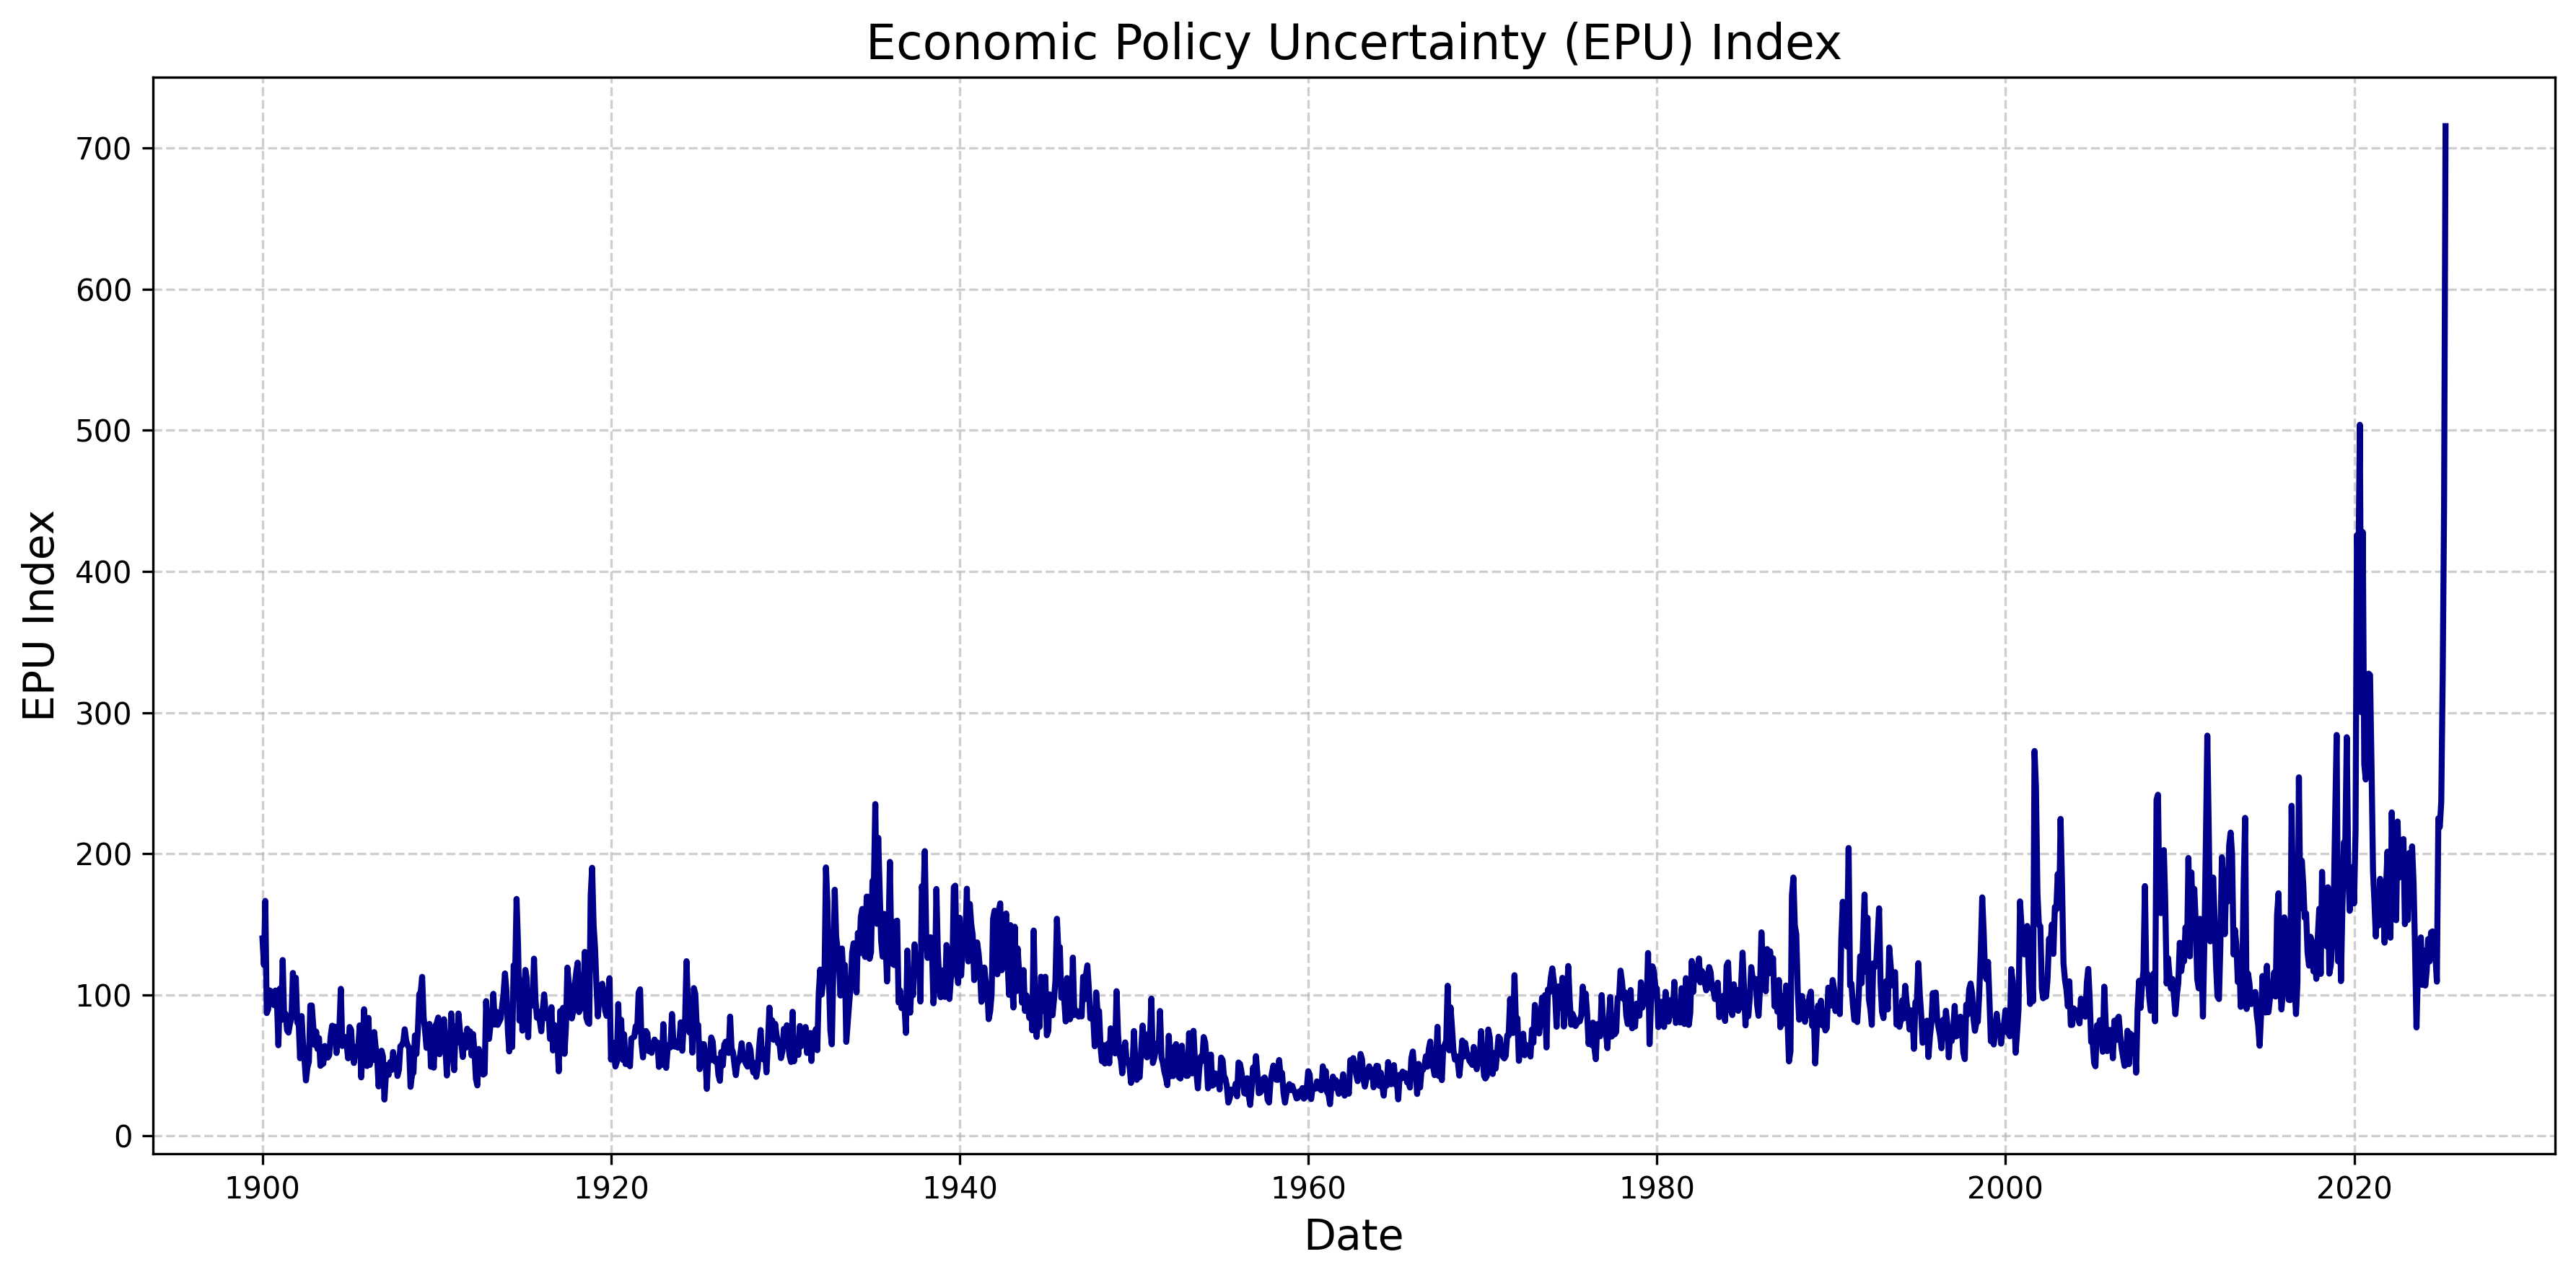
\includegraphics[width=1\linewidth]{Images/EPU_indicator_US.png}
  \caption{Economic Policy Uncertainty (EPU) index}
  \label{fig:EPU}
\end{figure}

\begin{figure}[h]
  \centering
  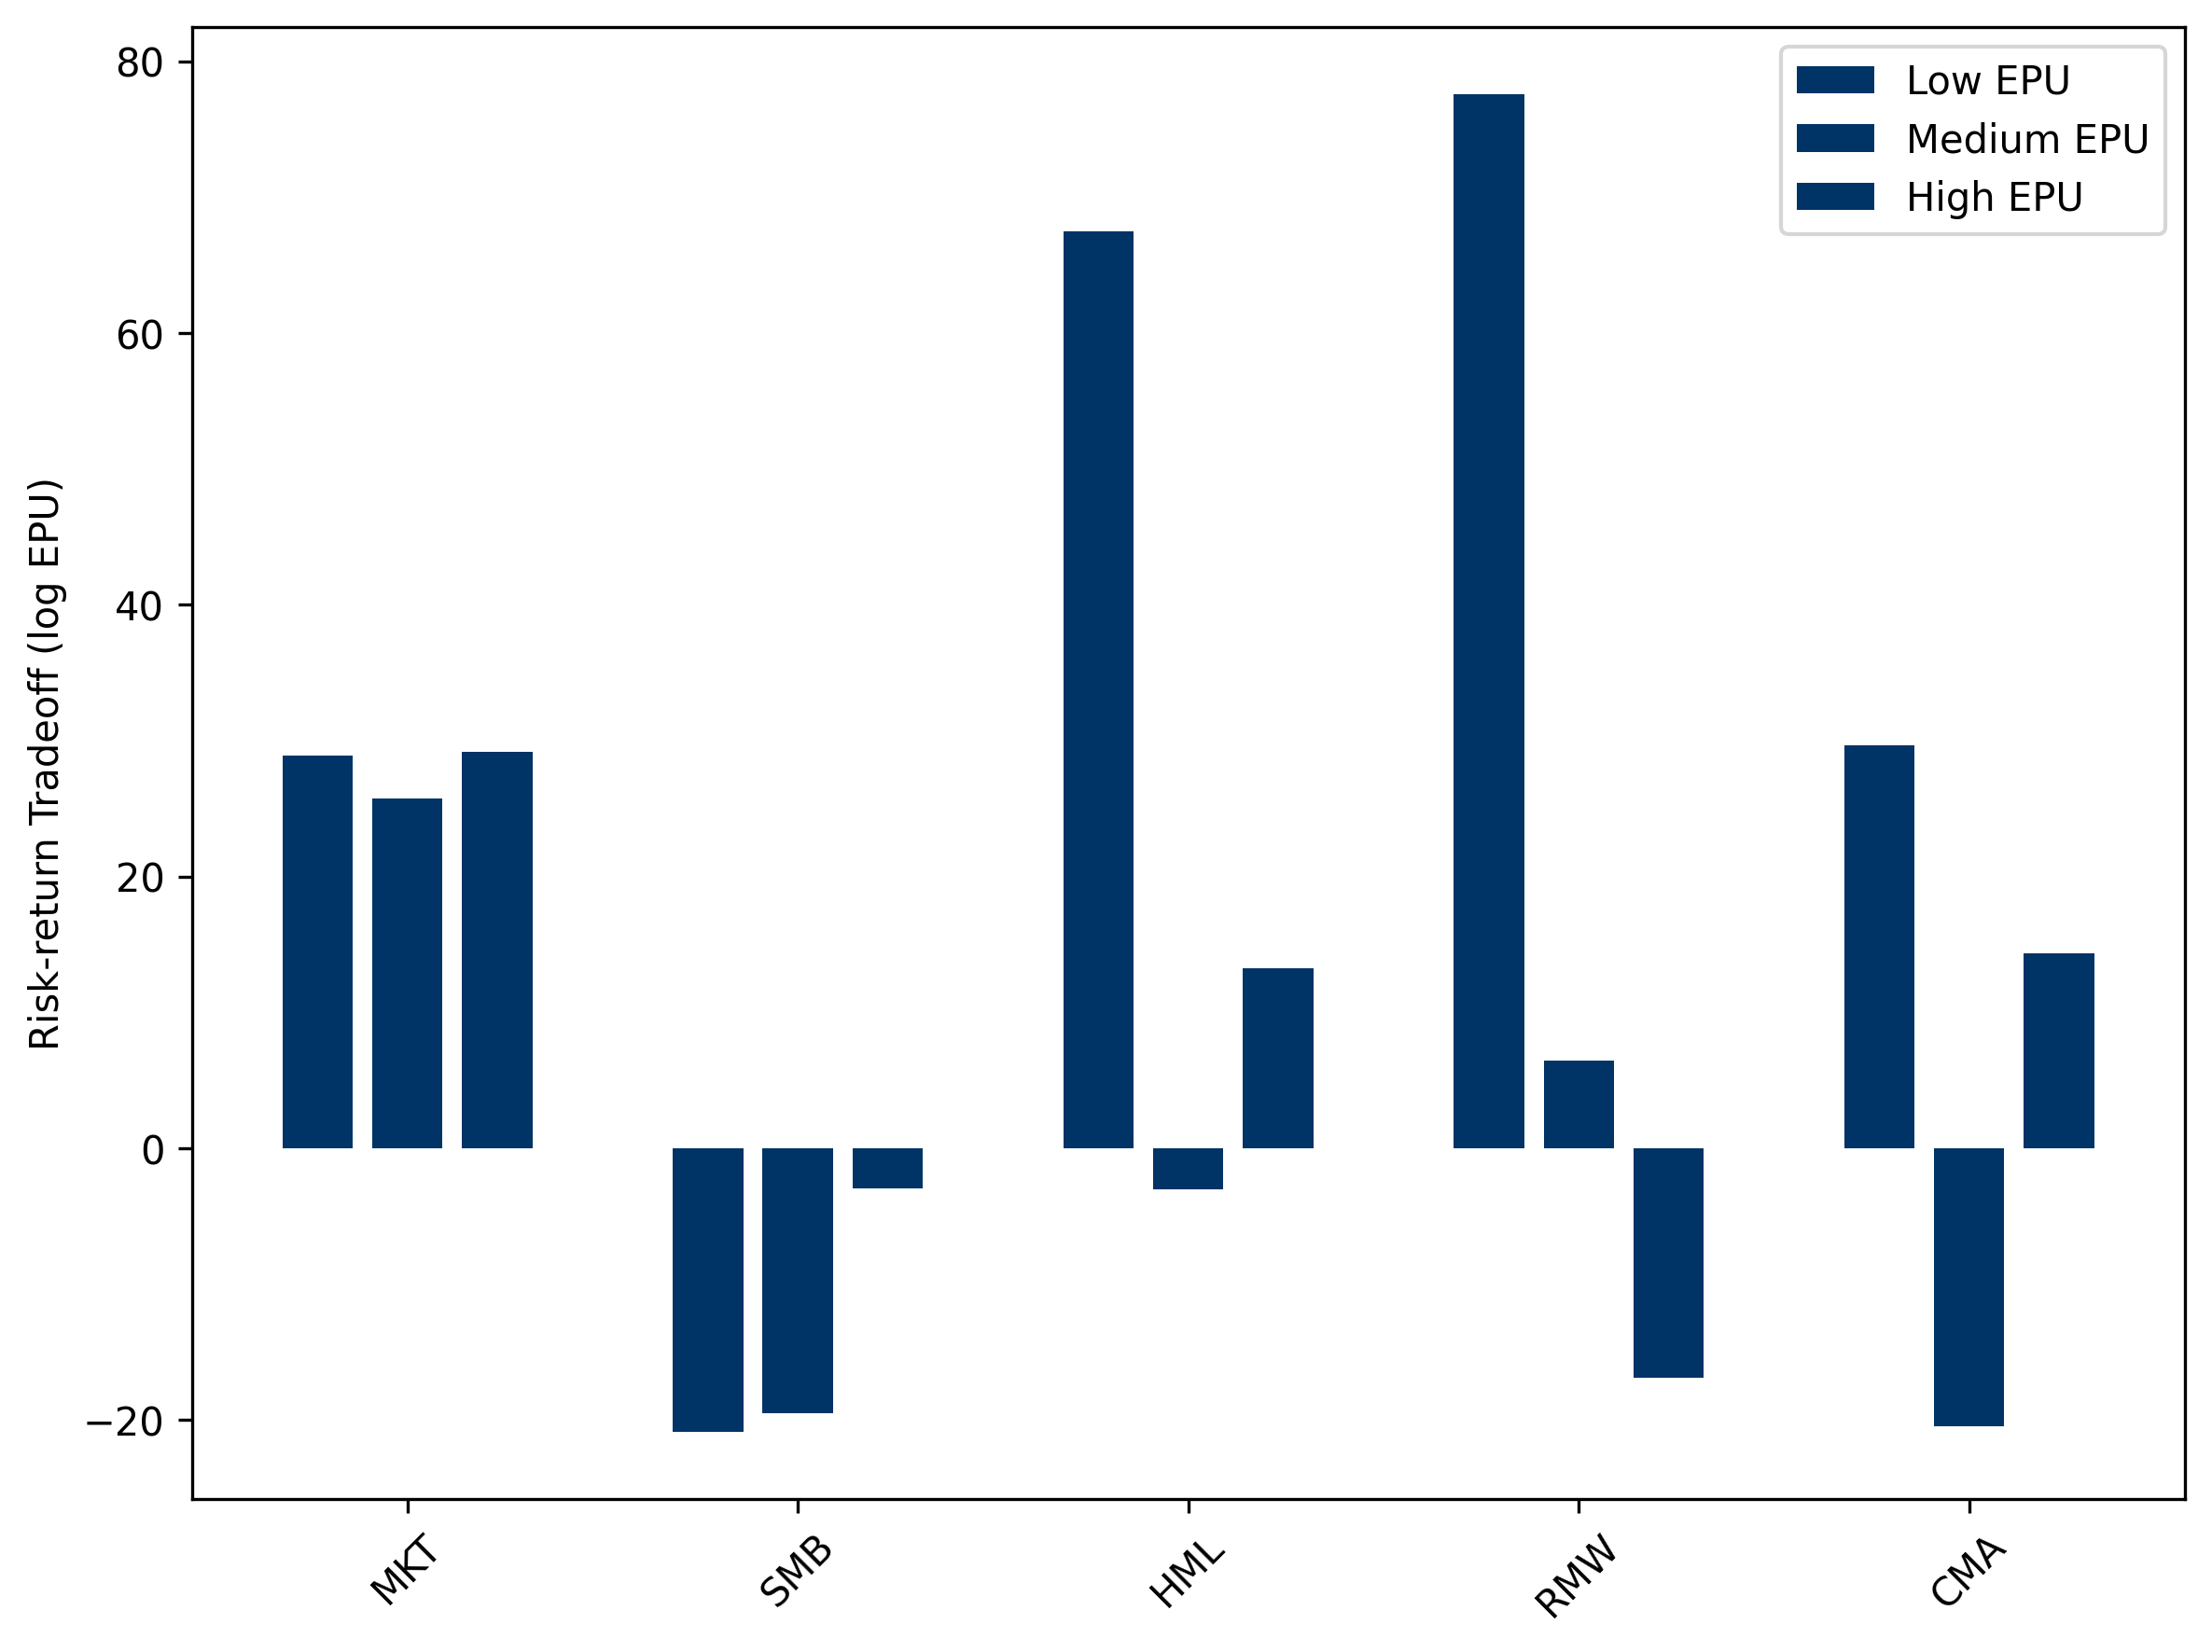
\includegraphics[width=1\linewidth]{Images/EPU-based buckets.png}
  \caption{EPU-based buckets}
  \label{fig:EPU-based buckets}
\end{figure}

\begin{figure}[h]
  \centering
  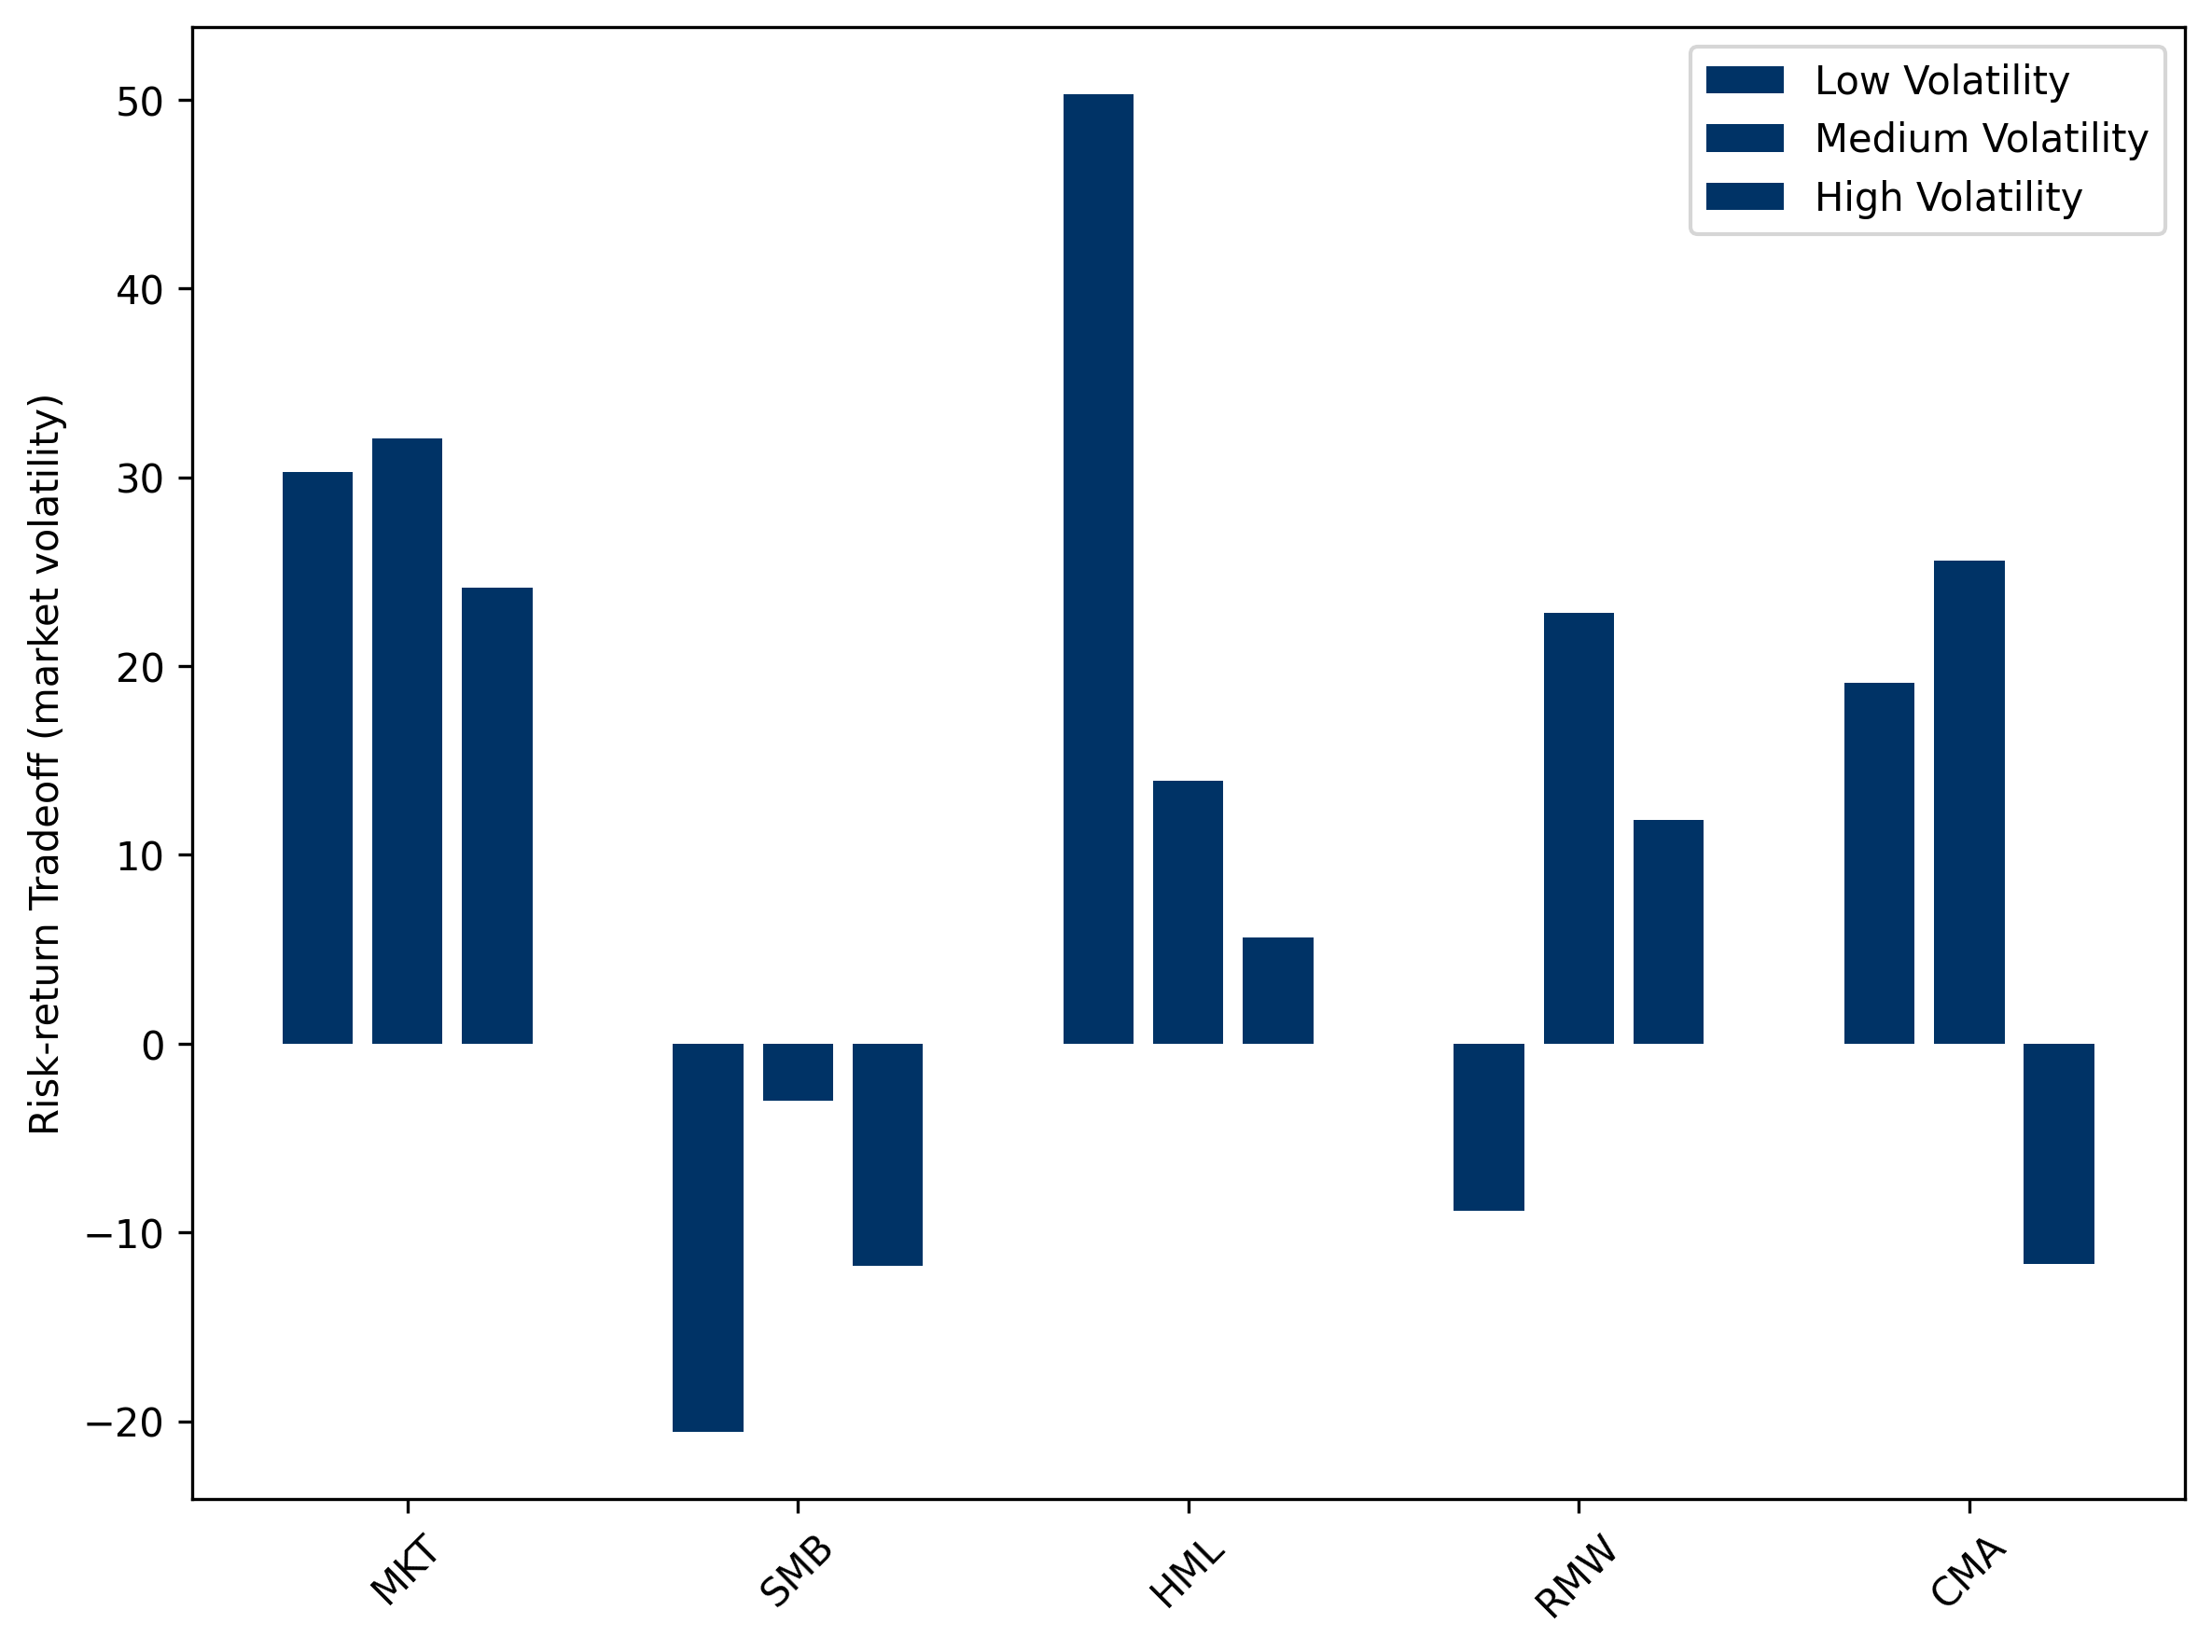
\includegraphics[width=1\linewidth]{Images/Volatility-based buckets.png}
  \caption{Volatility-based buckets}
  \label{fig:Volatility-based buckets}
\end{figure}
	% Appendix Title

%\input{Appendices/AppendixB} % Appendix Title

%\input{Appendices/AppendixC} % Appendix Title



\addtocontents{toc}{\vspace{2em}}  % Add a gap in the Contents, for aesthetics


%% ----------------------------------------------------------------

\appendix
\chapter*{Appendix: Tables and Figures}
\addcontentsline{toc}{chapter}{Appendix: Tables and Figures}
\section*{1 Tables}
\addcontentsline{toc}{section}{Tables}

\begin{table}[h!]
\centering
\begin{tabular}{lcccc}
\toprule
\textbf{Factor} & $\mu$ (in \%, annual) & $\sigma$ (in \%, annual) & Max (in \%) & Min (in \%) \\
\midrule
MKT & 7.078 & 16.185 & 11.3 & -17.4 \\
SMB & 1.592 & 8.740 & 6.2 & -11.2 \\
HML & 3.466 & 9.300 & 6.7 & -5.0 \\
RMW & 3.482 & 6.376 & 4.5 & -3.0 \\
CMA & 3.040 & 6.041 & 2.5 & -5.9 \\
\bottomrule
\end{tabular}
\caption{Summary statistics of factor returns. $\mu$ and $\sigma$ are annualized.}
\label{tab:factor_stats}
\end{table}

\begin{table}[htbp]
\centering
\caption{Sharpe ratios and Ledoit–Wolf tests (OOS, 1963–2024)}
\label{tab:sr_main}
\setlength{\tabcolsep}{6pt}
\renewcommand{\arraystretch}{1.15}
\begin{tabular}{lccccc}
\toprule
& MKT & SMB & HML & RMW & CMA \\
\midrule
\multicolumn{6}{l}{\emph{Sharpe ratios}}\\
SR: Original    & 0.397 & -0.256 & 0.259 & 0.178 & 0.242 \\
SR: Vol-Managed & 0.513 & -0.225 & 0.393 & 0.306 & 0.127 \\
SR: EPU-Managed & 0.515 & -0.236 & 0.307 & 0.236 & 0.197 \\
\midrule
$\Delta SR$ (Vol$-$Orig) & \valp{0.116}{0.969} & \valp{0.031}{0.977} & \valp{0.134}{0.965} & \valp{0.127}{0.980} & \valp{-0.115}{0.977} \\
$\Delta SR$ (EPU$-$Orig) & \valp{0.118}{0.940} & \valp{0.020}{0.982} & \valp{0.049}{0.998} & \valp{0.057}{0.950} & \valp{-0.045}{0.974} \\
$\Delta SR$ (EPU$-$Vol)  & \valp{0.002}{0.992} & \valp{-0.011}{0.982} & \valp{-0.085}{0.970} & \valp{-0.070}{0.950} & \valp{0.070}{0.965} \\
\bottomrule
\end{tabular}

\medskip
\footnotesize Notes: SRs are annualized. Differences tested with Ledoit–Wolf $Z$-test using 6-month block bootstrap with 10{,}000 repetitions. P-values in parentheses.
\end{table}

\begin{table}[htbp]
\centering
\caption{Alpha tests: managed vs. original factor (monthly OLS, NW $L\!=\!6$)}
\label{tab:alpha_main}
\setlength{\tabcolsep}{6pt}
\renewcommand{\arraystretch}{1.15}
\begin{tabular}{lccccc}
\toprule
& MKT & SMB & HML & RMW & CMA \\
\midrule
\multicolumn{6}{l}{\emph{Volatility-managed vs. Original}}\\
$\alpha$         & \valp{0.0032}{0.480} & \valp{-0.0018}{0.375} & \valp{0.0005}{0.816} & \valp{0.0000}{0.980} & \valp{0.0023}{0.131} \\
$R^2$            & 0.385 & 0.581 & 0.355 & 0.332 & 0.385 \\
RMSE             & 0.0091 & 0.0040 & 0.0048 & 0.0038 & 0.0032 \\
\midrule
\multicolumn{6}{l}{\emph{EPU-managed vs. Original}}\\
$\alpha$         & \valp{0.0059}{0.135} & \valp{-0.0013}{0.452} & \valp{0.0011}{0.540} & \valp{0.0009}{0.493} & \valp{0.0016}{0.300} \\
$R^2$            & 0.472 & 0.558 & 0.396 & 0.324 & 0.368 \\
RMSE             & 0.0076 & 0.0038 & 0.0042 & 0.0036 & 0.0031 \\
\bottomrule
\end{tabular}

\medskip
\footnotesize Notes: $\alpha$ in monthly units. Newey–West standard errors with 6 lags. P-values in parentheses. Sample size $N = 617$ months.
\end{table}

\clearpage
\section*{2 Figures}
\addcontentsline{toc}{section}{Figures}

\begin{figure}[h]
  \centering
  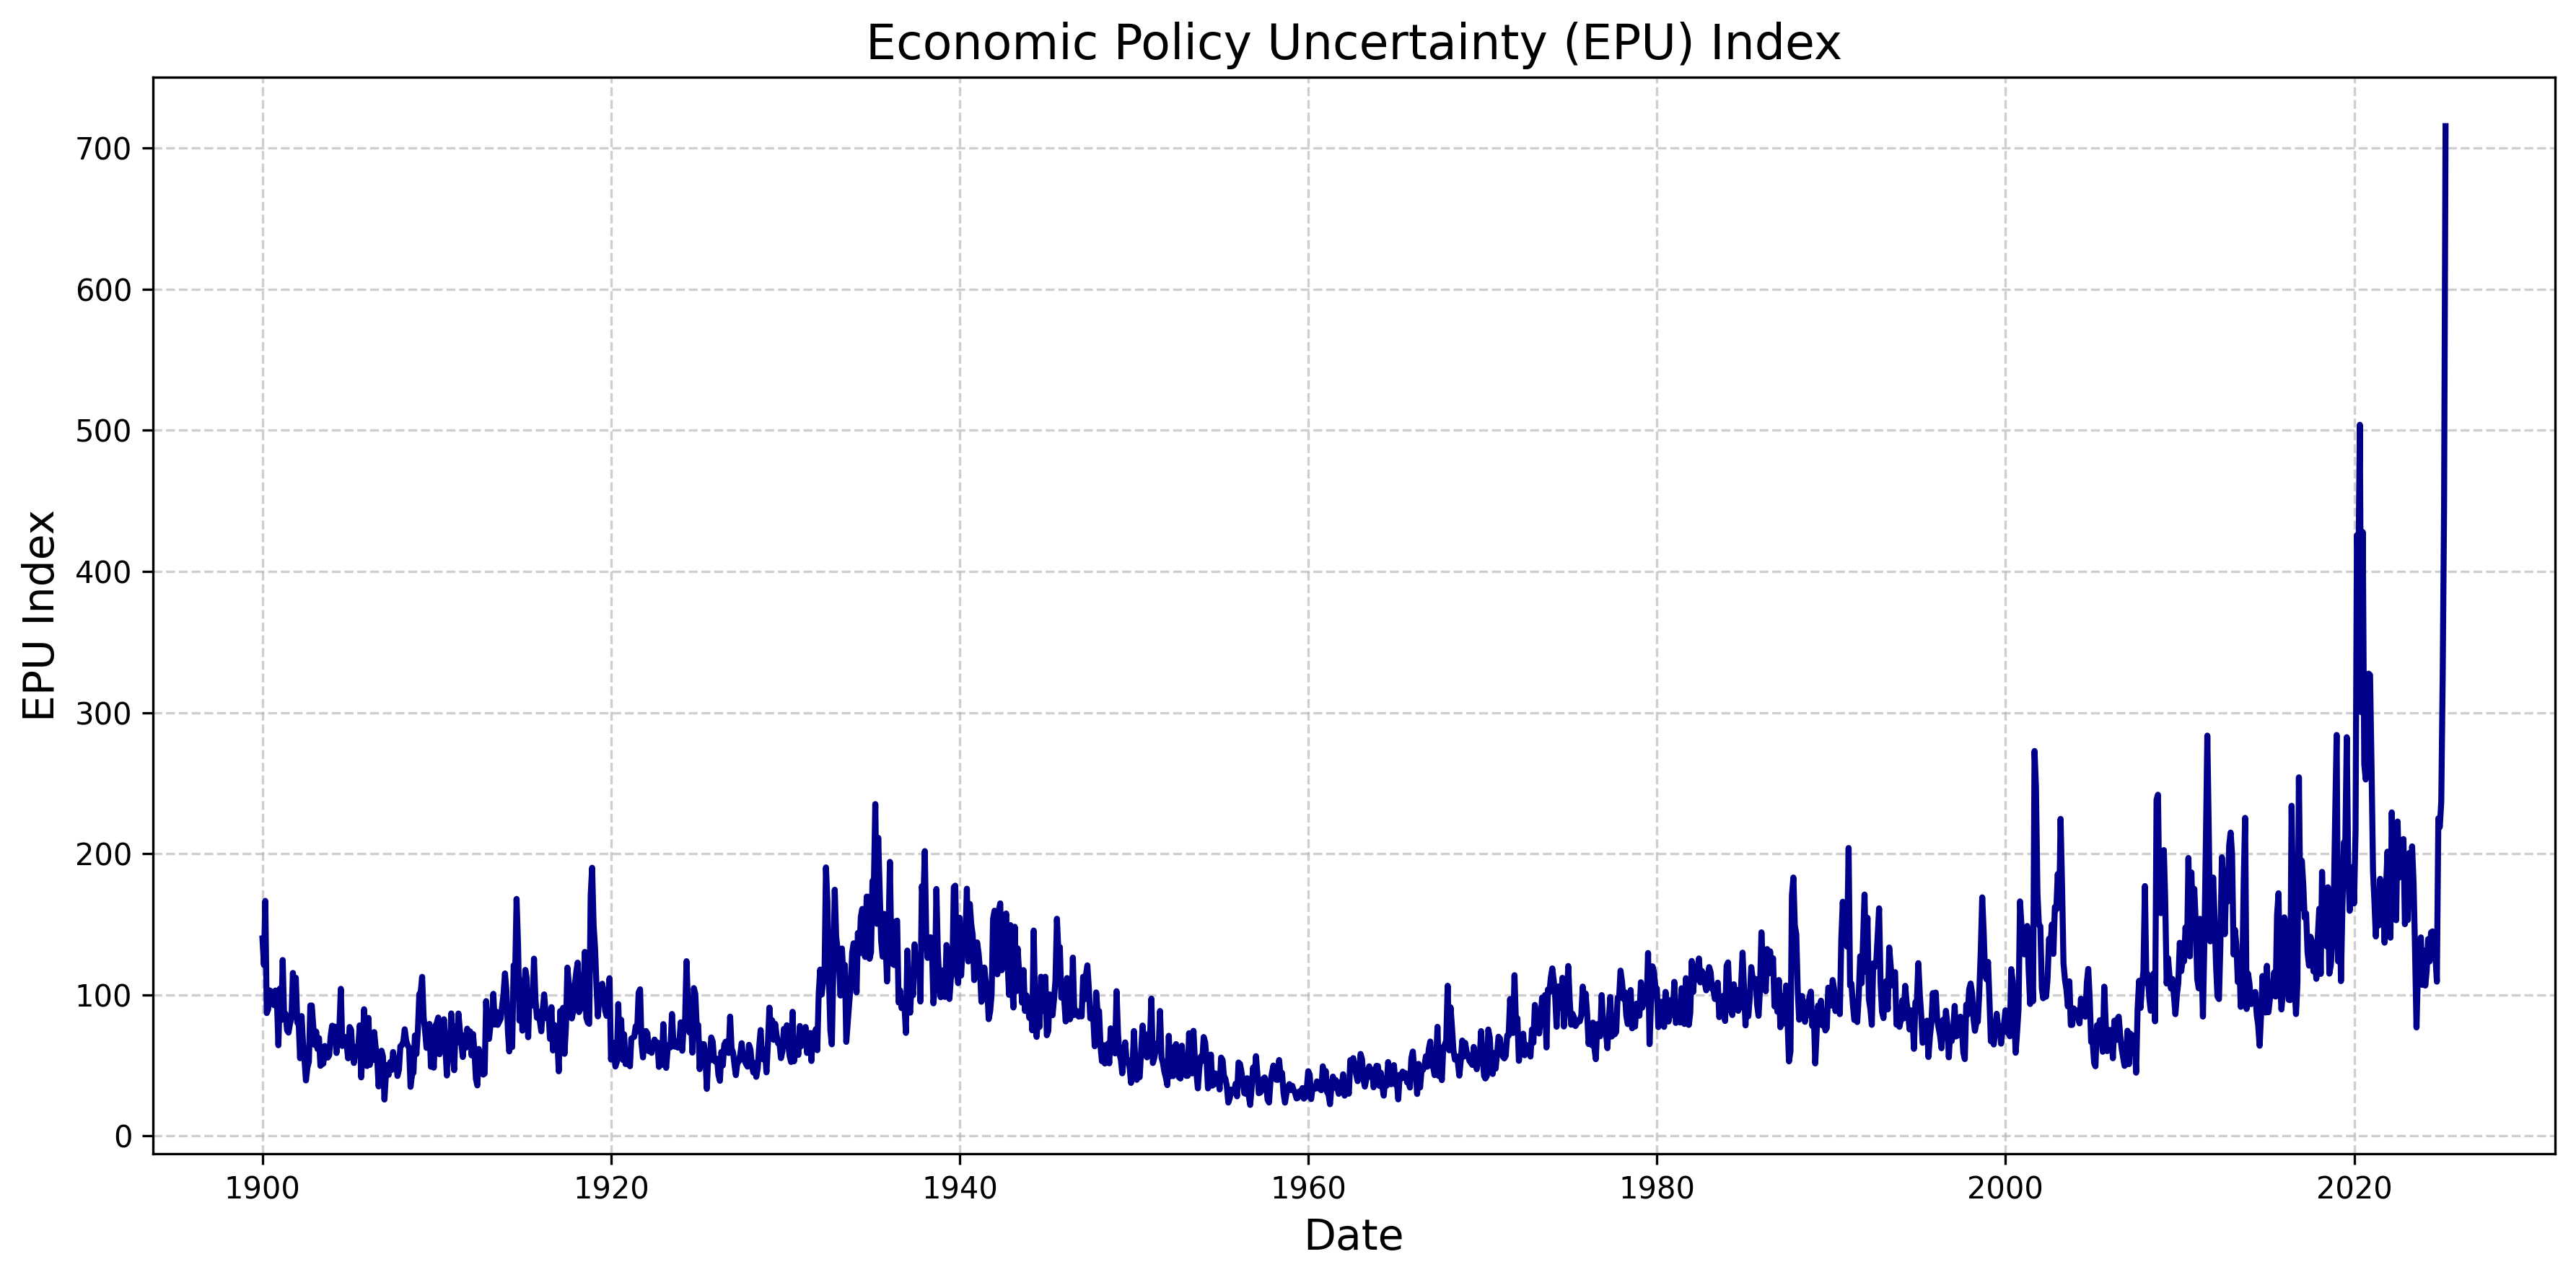
\includegraphics[width=1\linewidth]{Images/EPU_indicator_US.png}
  \caption{Economic Policy Uncertainty (EPU) index}
  \label{fig:EPU}
\end{figure}

\begin{figure}[h]
  \centering
  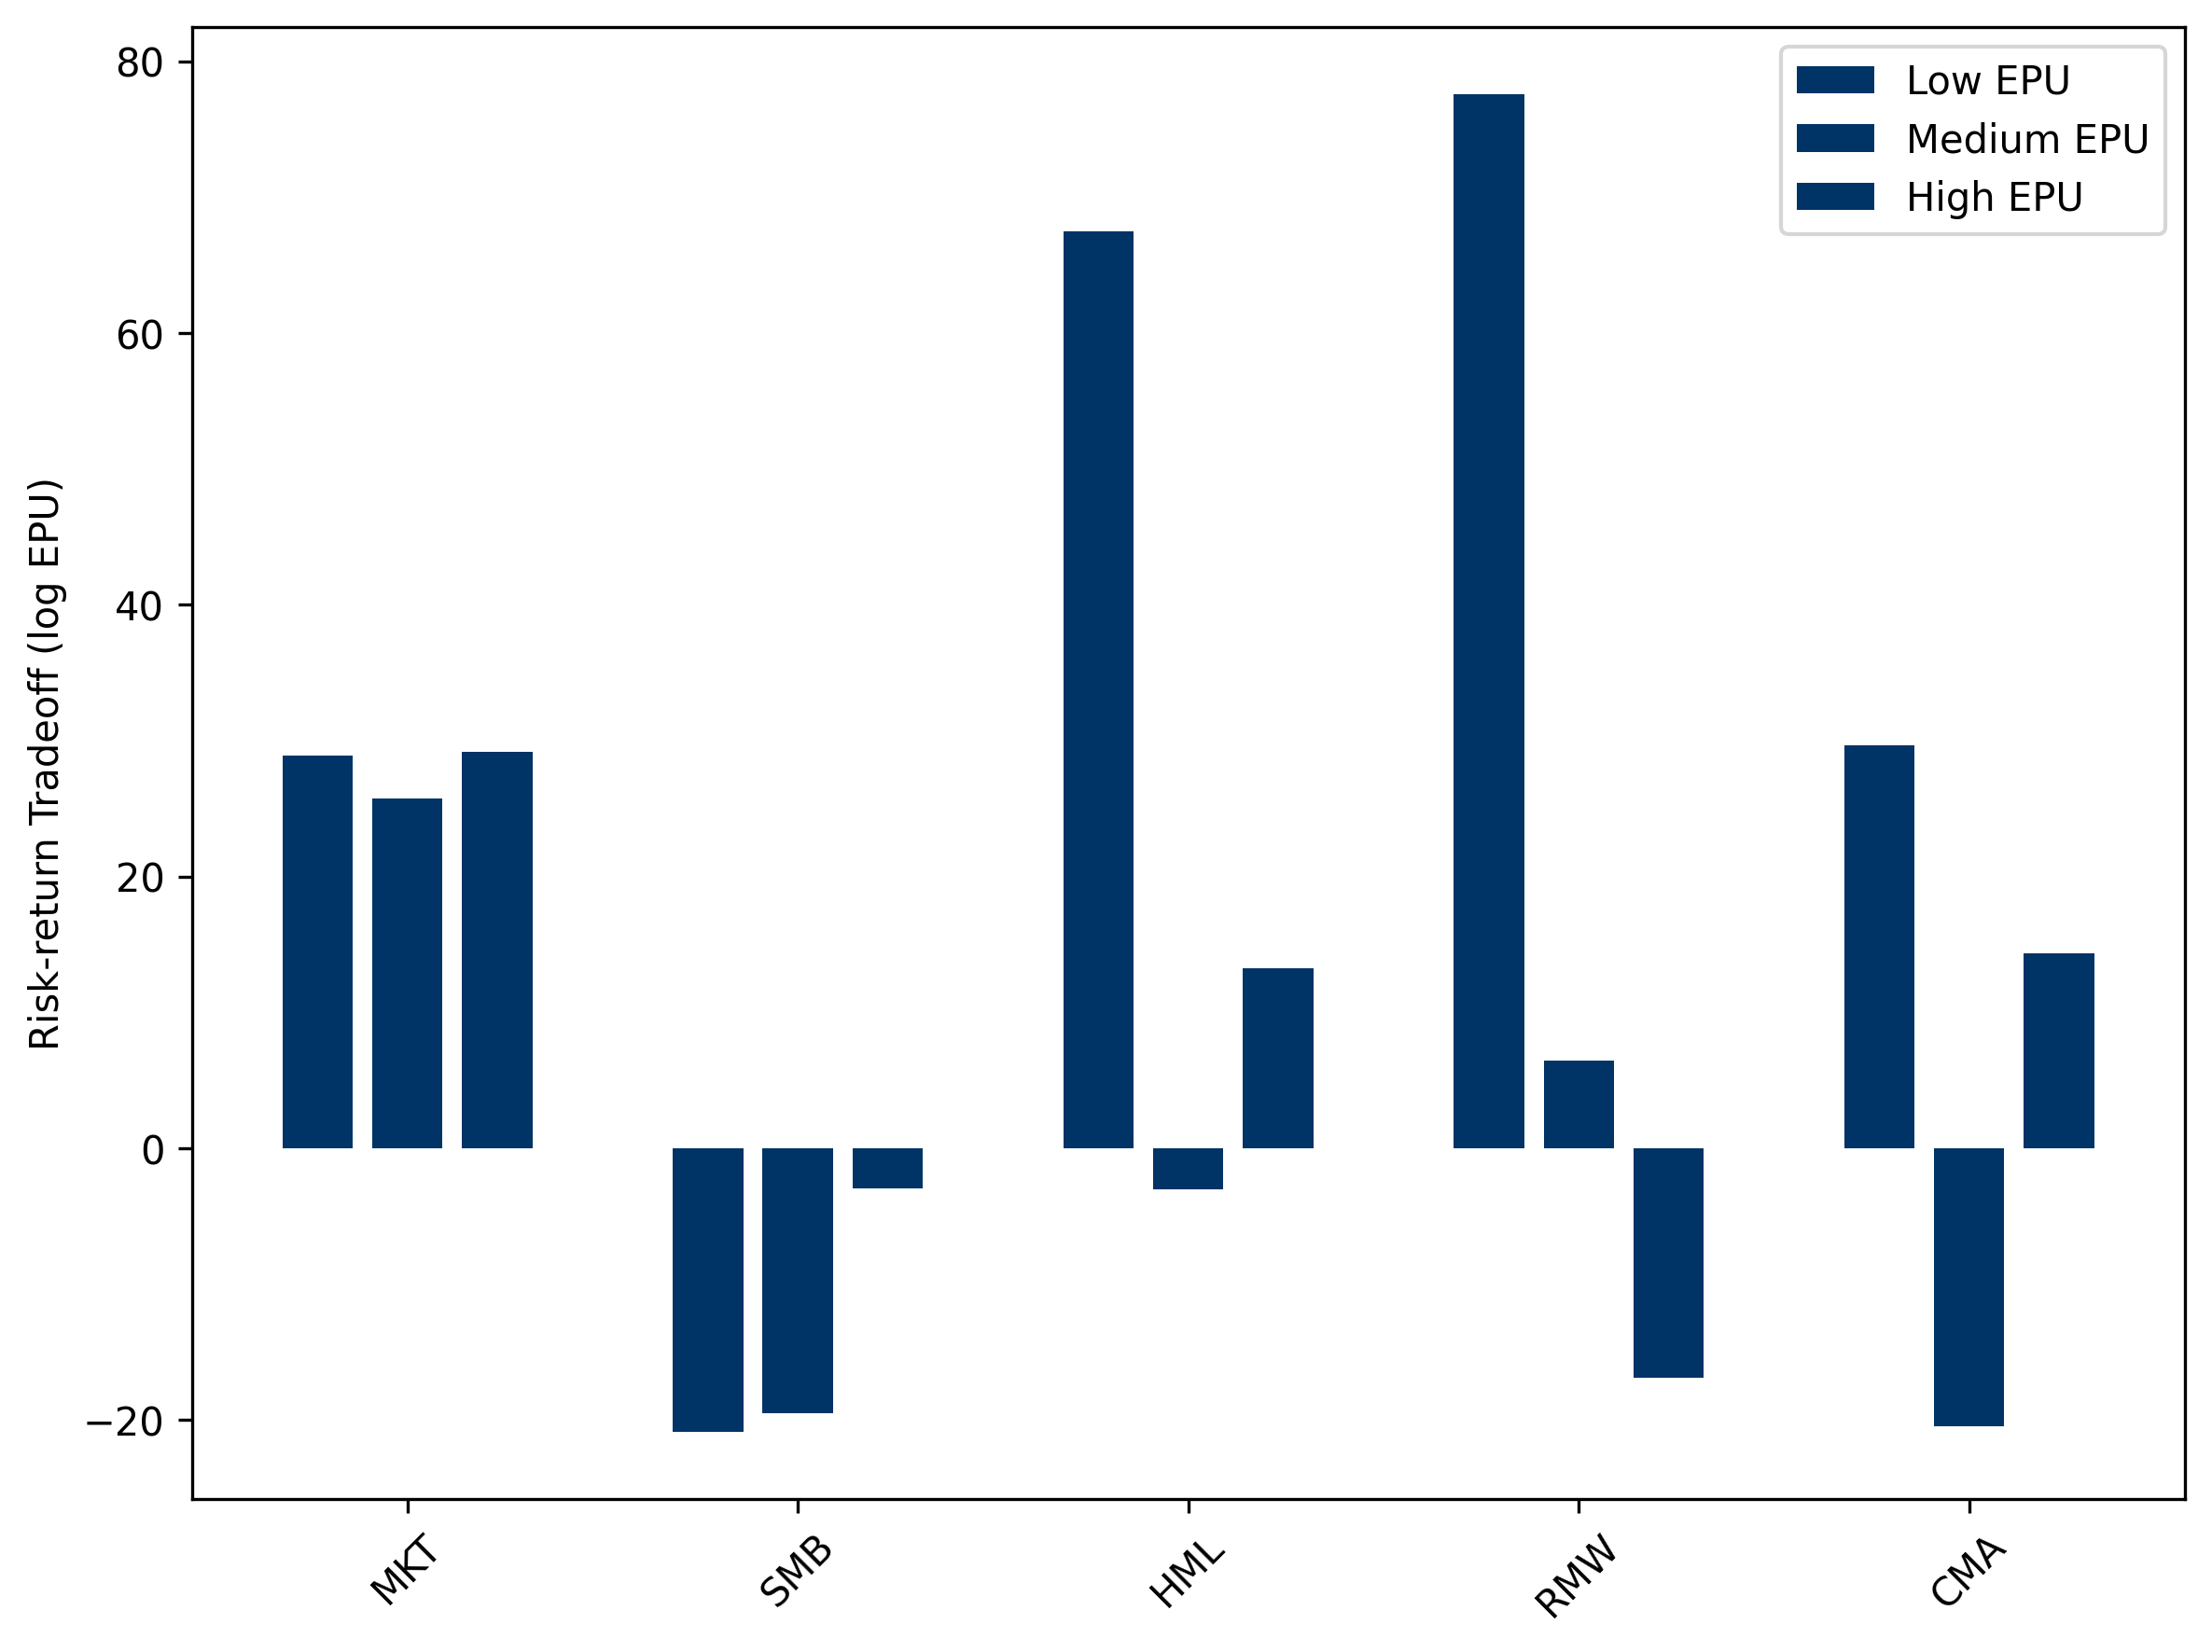
\includegraphics[width=1\linewidth]{Images/EPU-based buckets.png}
  \caption{EPU-based buckets}
  \label{fig:EPU-based buckets}
\end{figure}

\begin{figure}[h]
  \centering
  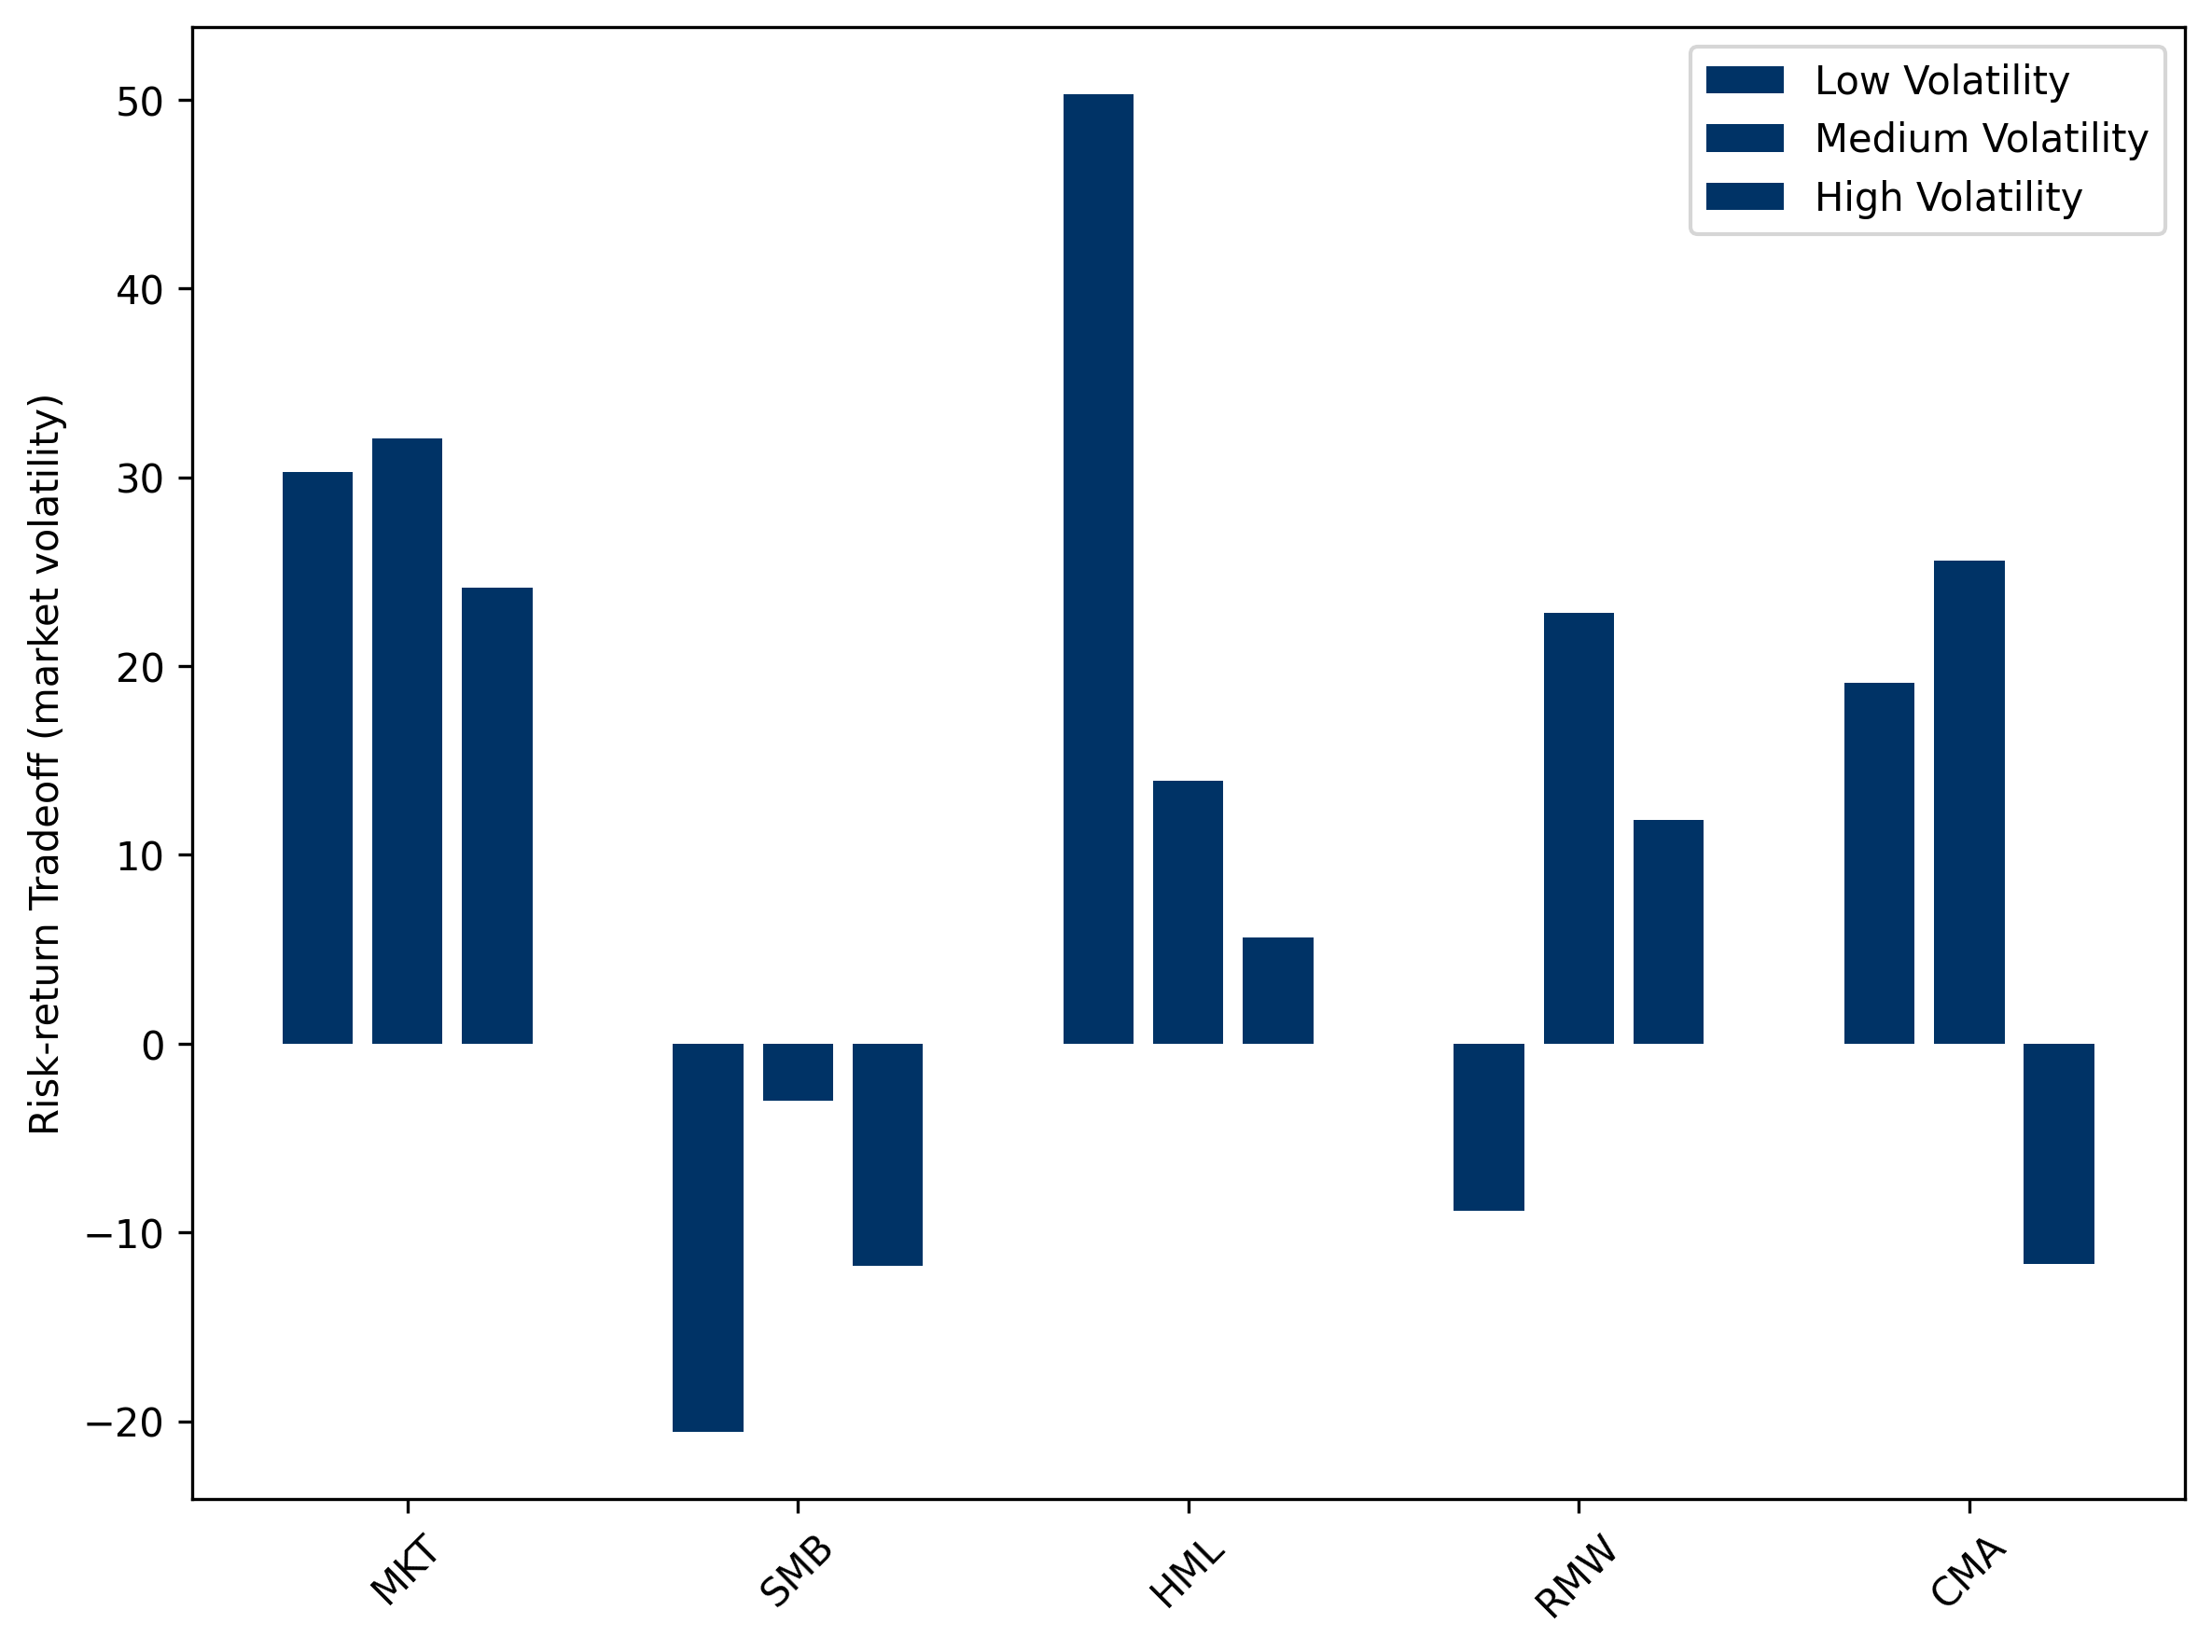
\includegraphics[width=1\linewidth]{Images/Volatility-based buckets.png}
  \caption{Volatility-based buckets}
  \label{fig:Volatility-based buckets}
\end{figure}


% потом уже библиография
\bibliographystyle{unsrtnat}
\bibliography{Bibliography}



\end{document}  % The End
%% ----------------------------------------------------------------